\section{Introduction}
Many websites \citep{codesansar2021} provide tools to determine an LU  decomposition of a matrix; however, none of them can decompose \emph{all} matrices. 
Using code, we developed a GeoGebra applet that can decompose square matrices for those that can be factored and decompose ``nearby" matrices without an LU decomposition using perturbation. In this paper, we first present conditions for a  matrix to have a unique LU decomposition. Several examples are included to illustrate this theorem.  Next, we state and prove special cases for matrices with infinitely many and no LU factorizations.  \\


 
%: SECTION - LU DECOMPOSITION
\section{Mathematics}\label{sec:lu}
Here is some mathematics.  For $A \in M_n$, the factorization $A = LU$, where $L$ is unit lower triangular and $U$ is upper triangular,  is called the \textit{LU decomposition}, or \textit{LU factorization}.  We can use such a factorization, when it exists, to solve the system $A {\bf x} = {\bf b}$ by first solving for the vector $\bf{y}$ in $L {\bf y} = {\bf b}$ 
and then solving 
$
U {\bf x} = {\bf y}
$. 
However, not every $n \times n$ matrix $A$ has an LU decomposition.  The following theorem provides conditions for the existence and uniqueness of an LU decomposition of a $n \times n$ matrix.  A proof can be found in \citet[p. 160]{johnson1985matrix}.  An equation is given by \cite{strang1993introduction}, 

\begin{equation}\label{eqn:quad}
x = \frac{-b \pm \sqrt{b^2 - 4ac}}{2a}
\end{equation}
  
%: EXAMPLE 1
\begin{example}\normalfont
The $3 \times 3$ matrix  
$A =  \begin{bmatrix}
1 & 5 & 1\\
1 & 4 & 2\\
4 & 10 & 2\\
\end{bmatrix}
$
has all non-zero principle minors, $A_1, A_2$ and $A_3$.  Therefore,  there is a unique LU factorization with both $L$ and $U$ nonsingular given by 
\end{example}
\[
\begin{bmatrix}
1 & 5 & 1\\
1 & 4 & 2\\
4 & 10 & 2\\
\end{bmatrix}
=
\begin{bmatrix}
1 & 0 & 0\\
1 & 1 & 0\\
4 & 10 & 1\\
\end{bmatrix}
\begin{bmatrix}
1 & 5 & 1\\
0 & -1 & 1\\
0 & 0 & 12\\
\end{bmatrix}.
\]
 
 
  
 
\section{Definition, Theorem, Corollary, Example}


\begin{definition}
Definitions are if and only if statements.  
\end{definition}

\begin{verbatim}
\begin{definition}
Definitions are if and only if statements.  
\end{definition}
\end{verbatim}

%: THEOREM: Infinite LU Factorizations
\begin{theorem}[Matrices with Infinitely Many LU Factorizations]
{For $A \in M_n$, if two or more of any first $(n-1)$ columns are linearly dependent or any of the first $(n-1)$ columns are 0, then $A$ has infinitely many LU factorizations.}
\end{theorem}

%: proof
\begin{proof} We will prove only for the the case when $A \in M_3$. \\
 \begin{align} 
&dm + r = e  \Rightarrow r = e-dm \label{eqn:1}\\
&dn + rp = f \Rightarrow p=\frac{f-dn}{r} \label{eqn:2}\\
&gm + s = h \Rightarrow s = h - gm \label{eqn:3}\\
&gn + sp + t = i \Rightarrow t  = i-sp-gn \label{eqn:4}
\end{align}
 
\end{proof}
% ----------------------------------------- %

 

 







 









 \section{Lists}
 NAGJ uses the \verb|outline| package.  
 
 % Enumeration
 \subsection{Enumerated List}
 The following code produces an enumerated list.
 
% Verbatim Outline
\begin{verbatim}
\begin{outline}[enumerate]
     \1 First Level
          \2 Second level
               \3 Third level
\end{outline}
 \end{verbatim}
 
 % Outline
 \begin{outline}[enumerate]
 	\1 First Level
		\2 Second level
			\3 Third level
\end{outline}
 
 
 
 % Itemize
 \subsection{Itemized List}
 The following code produces an itemized list.
 
% Verbatim Outline
\begin{verbatim}
\begin{outline}
     \1 First item
          \2 Second level item
               \3 Third level sub-item
\end{outline}
 \end{verbatim}
 
 % Outline
 \begin{outline}
 	\1 First Level
		\2 Second level
			\3 Third level
\end{outline}









% Examples
\section{Examples}\label{ex:x1}
Here is an example of an example.


\begin{example}
Let  $\{1,2,3\}$ and $\{2,1,3\}$ be two lists of integers.  Then, to check if the two lists are equal we would have,   
	\begin{center}
		\texttt{ \{1,2,3\} == \{2,1,3\} }.
	\end{center}\label{ex:equallists}
\end{example}


\begin{verbatim}
\begin{example}
Let  $\{1,2,3\}$ and $\{2,1,3\}$ be two lists of integers.  Then, to check if the two lists are equal we would have,   
	\begin{center}
		\texttt{ \{1,2,3\} == \{2,1,3\} }.
	\end{center}\label{ex:equallists}
\end{example}
\end{verbatim}











%: SECTION - Tables and Figures
\section{Tables and Figures}
 
 
 \subsection{Figures}
  Figures should be high quality (1200 dpi for line art, 600 dpi for grayscale and 300 dpi for color, at the correct size). Figures should be supplied in one of our preferred file formats: EPS, PS, JPEG, TIFF, or Microsoft Word (DOC or DOCX) files are acceptable for figures that have been drawn in Word. For information relating to other file types, please consult our Submission of electronic artwork document.
  
 \begin{figure}[h!] %  figure placement
    \centering
    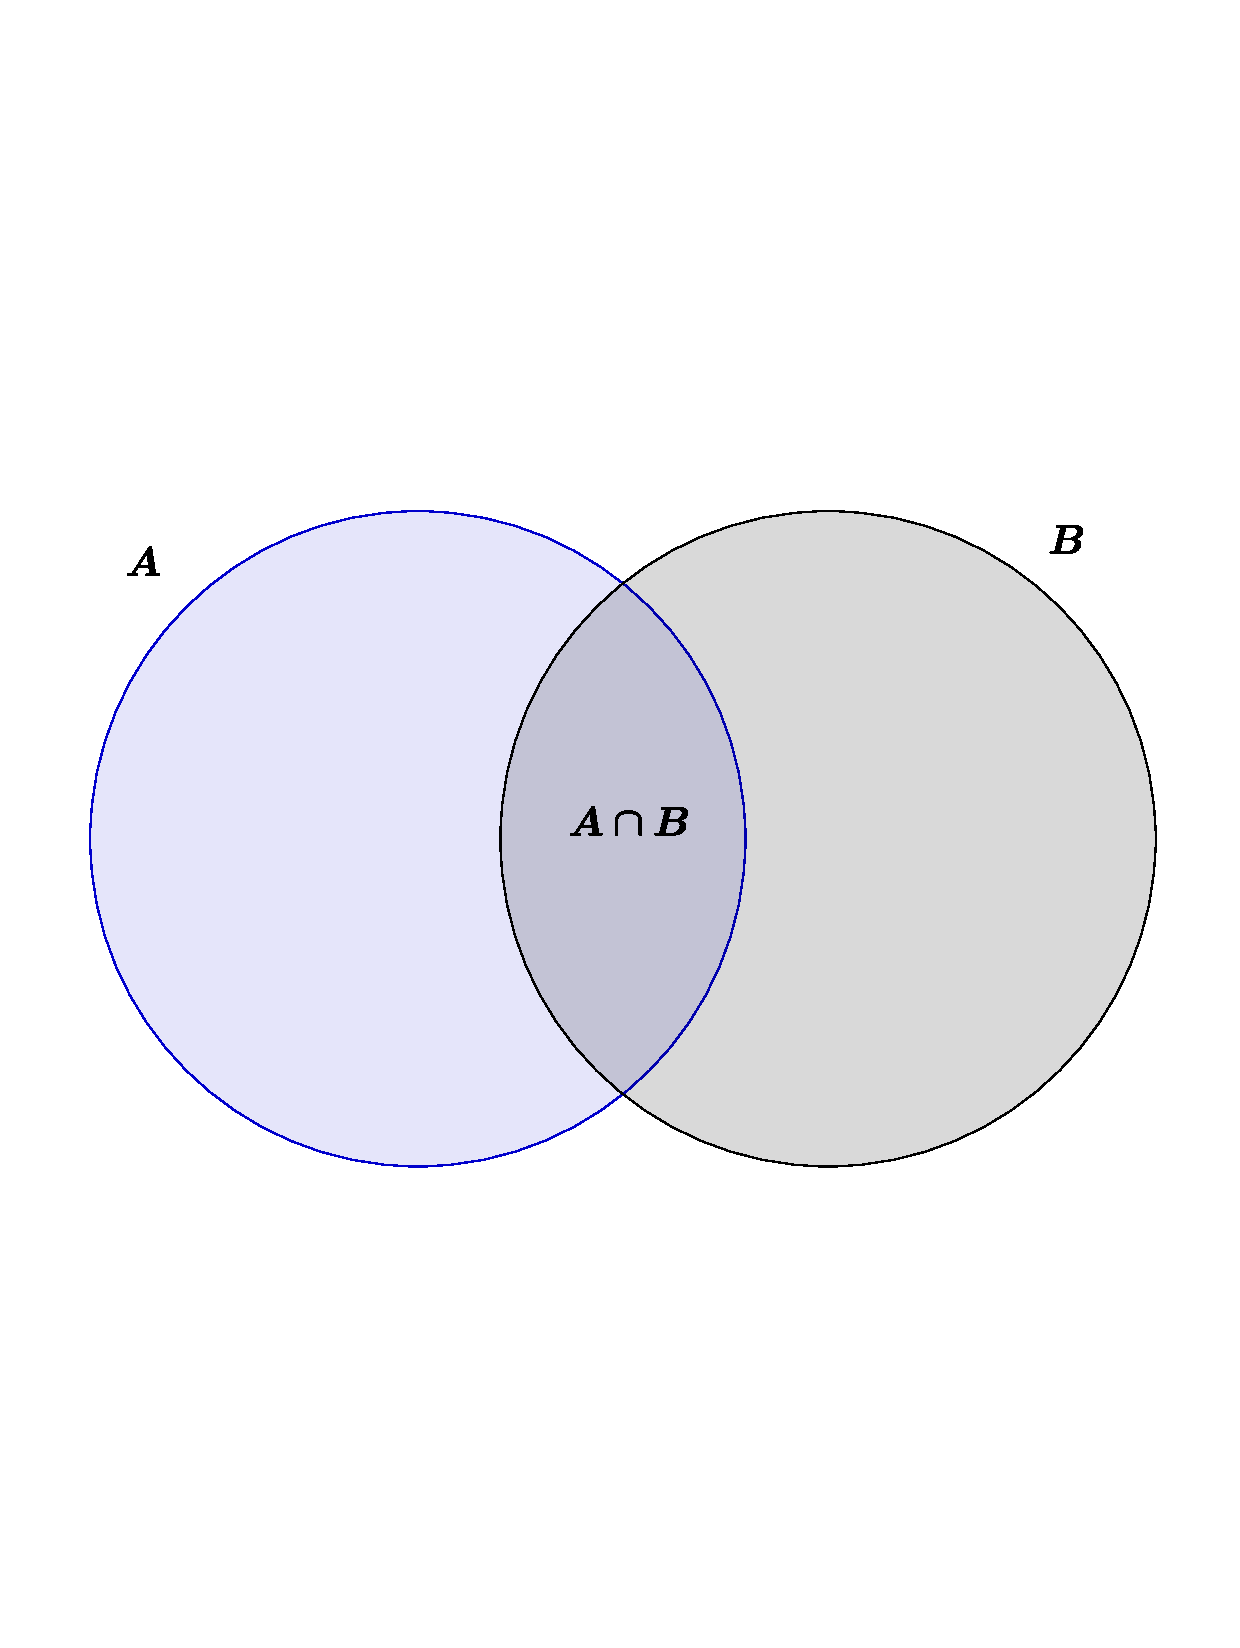
\includegraphics[scale=0.5]{figs/venn.pdf} 
    \caption{Provide a short caption description.}
    \label{fig:number}
 \end{figure}
 
 
 
 \subsection{Tables}
We use the \texttt{booktabs} package.  Tables should present new information rather than duplicating what is in the text. Readers should be able to interpret the table without reference to the text. Please supply editable files.




\section{Cross Reference}
Figures, tables, and equations should be labeled (\texttt{label}) then referenced using the \texttt{ref}. 
